\chapter[Model for Near-Field Radiative Heat Transfer Between Spherical Bodies][Model for Near-Field Radiative Heat Transfer Between Spherical Bodies]{Model for Near-Field Radiative Heat Transfer Between Spherical Bodies} \label{ch:model} \allowdisplaybreaks

\begin{quote}
    We choose to work with spheres not because they are easy, but because they are hard; because that goal will serve to organize and measure the best of our energies and skills, because that challenge is one that we are willing to accept, one we are unwilling to postpone, and one we intend to win, and the others, too. \sourceatright{John F. Kennedy, probably}
\end{quote}

\section{Introduction}
%
In this chapter, we will develop a model for NFRHT between spherical objects, and between a spherical object and its environment. Specifically, we will examine the case of a linear chain of spheres, a chain in which the centers of every sphere lie on a common axis. I published this work in Refs. \citenum{Czapla2017} and \citenum{Czapla2018}. Spheres are an important geometry to investigate because of their numerous useful properties: they are compact objects with a convenient coordinate system, they have rotational symmetry, in the limit as one sphere is much larger than the second you recover a sphere-plane geometry, small spheres can approximate dipoles, etc. For these reasons and more, a model of NFRHT involving spheres is an attractive tool to add to the the toolbox of the NFRHT community.

I will proceed as follows: first, I will provide the geometrical definitions required to describe a linear chain of spheres. Next, I will mathematically define vector spherical waves and demonstrate how to translate them between coordinate systems. After that, I will use the vector spherical waves to construct the DGFs of the system. Finally, I will use the DGFs to solve for the transmissivity which describes sphere-sphere and sphere-environment NFRHT.

\section{Geometry of Linear Chain}
%
The configuration of the chain of spheres is shown in Fig. \ref{fig:Chain_Geometry}. In Fig. \ref{fig:Chain_Geometry}A, an individual sphere, labeled sphere $i$, is depicted. Sphere $i$ has an outer radius, $\rho_{i}$. Internally, it may be homogeneous or composed of spherically symmetric layers. Coordinate system $i$ is fixed to the center of sphere $i$. Any position vector, $\boldsymbol{r}$ or $\widetilde{\boldsymbol{r}}$, when written in coordinate system $i$, is denoted $\boldsymbol{r}_{i}$ or $\widetilde{\boldsymbol{r}}_{i}$, respectively. 

Figure \ref{fig:Chain_Geometry}B depicts a section of a linear chain of $N_{s}$ spheres, which is embedded in free space (referred to as region $f$). The $z$-axis of coordinate system $i$ ($1 \le i \le N_{s}$) is aligned down the central axis of the chain. The $x$-axes of all coordinate systems are parallel, and similarly so are the $y$-axes.

The spheres are numbered $1$ through $N_{s}$, such that their labels increase along the positive $z$-direction (of any coordinate system). Any two spheres, $i$ and $j$, are separated by center-to-center distance $d_{i,j}$ and the minimum separation between them is $D_{i,j} = | d_{i,j} | - \rho_{i} - \rho_{j}$ (not depicted explicitly in Fig. \ref{fig:Chain_Geometry}). The sign of $d_{i,j}$ is positive if $j > i$ and negative if $j < i$.

\begin{figure}
\centering
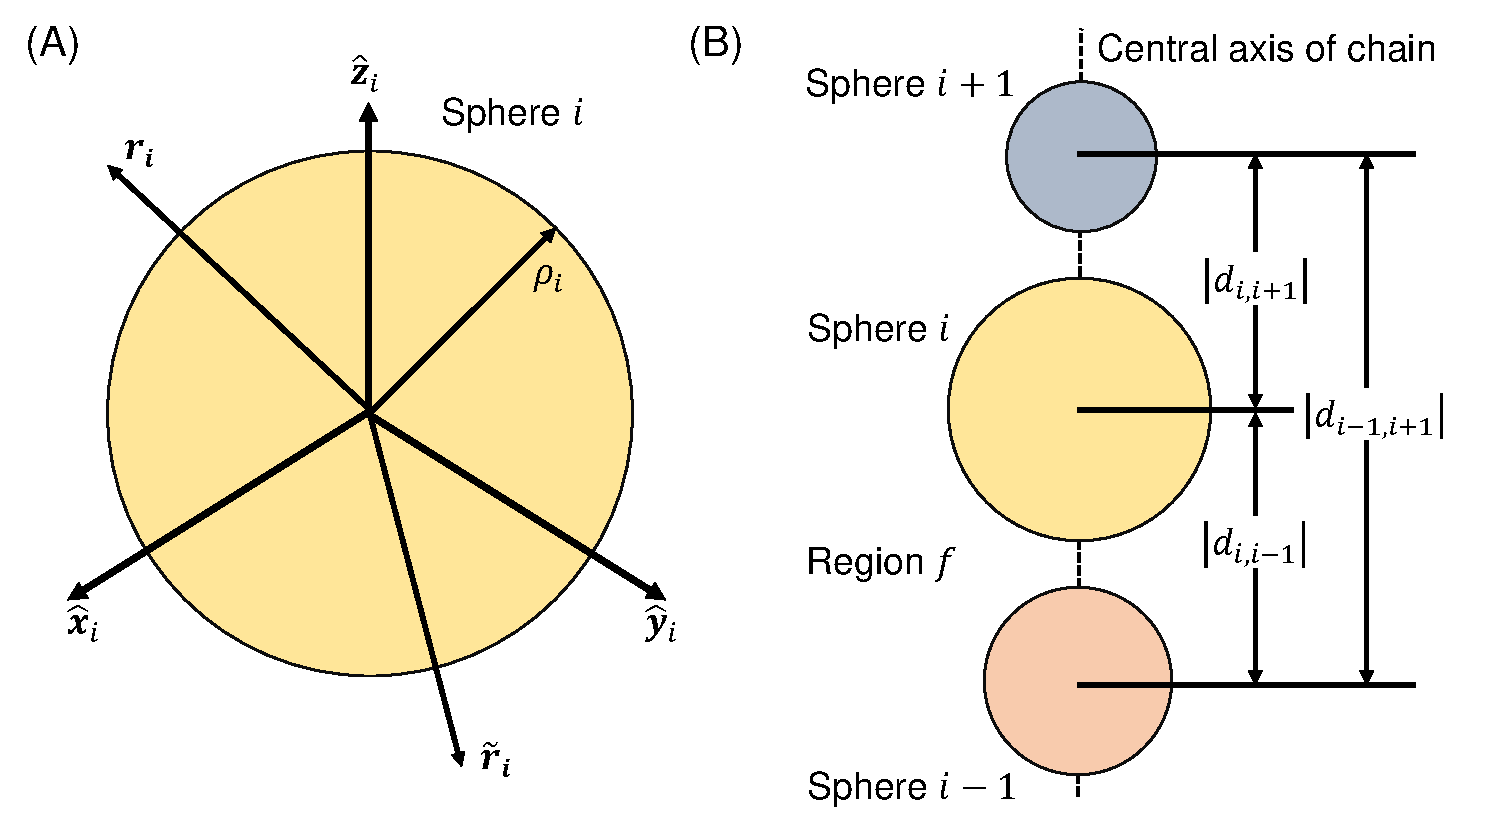
\includegraphics[width=0.8\textwidth]{./Figures/Chain_Geometry.pdf}
\caption{\label{fig:Chain_Geometry}Configuration of spheres in chain. (A) Single sphere $i$ and its associated coordinate system. (B) Section from a linear chain of spheres embedded in region $f$.}
\end{figure}


\section{Spherical Waves}

\subsection{Spherical Coordinate System}
Throughout this chapter, we will be working extensively in spherical coordinates. The convention used to define unit vectors in spherical coordinates varies by field, so a depiction of the convention used henceforth is given as Fig. \ref{fig:SphericalCoordinates}. In our system, $\phi$ defines the azimuthal direction and $\theta$ defines the polar (zenith) angle. The radial distance from the origin is given by $r$.
%
\begin{figure}
\centering
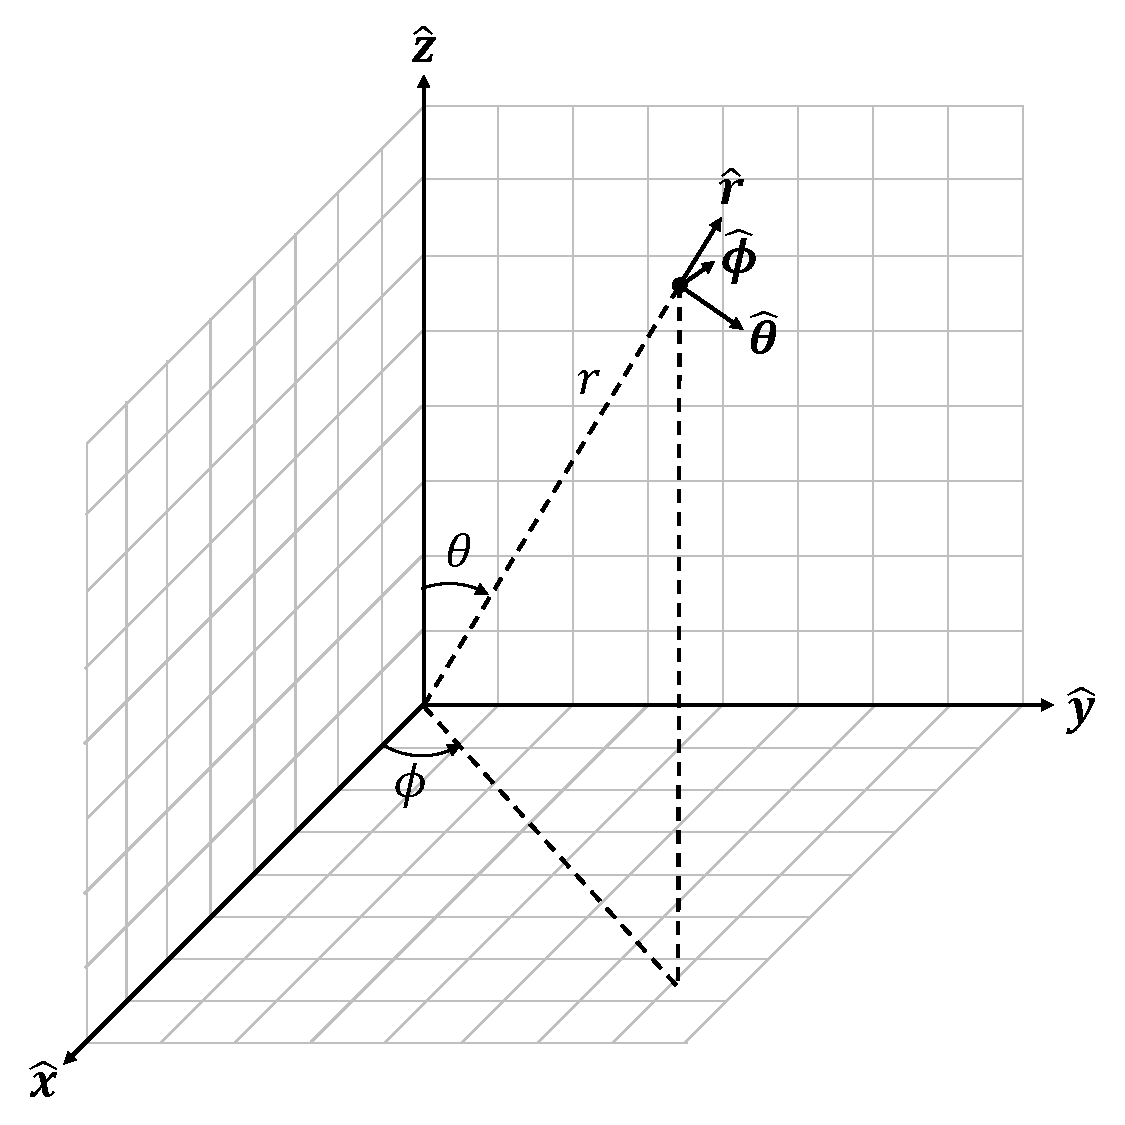
\includegraphics[width=0.8\textwidth]{./Figures/SphericalCoordinates.pdf}
\caption{\label{fig:SphericalCoordinates}Spherical coordinate system convention used in this work.}
\end{figure}

\subsection{Vector Eigenfunctions}
%
When expressed in a spherical coordinate system, the solutions to the homogeneous vector Helmholtz equation are vector spherical waves (VSWs). Three such VSWs exist: $\boldsymbol{L}_{lm}^{(p)}(k\boldsymbol{r})$, $\boldsymbol{M}_{lm}^{(p)}(k\boldsymbol{r})$, and $\boldsymbol{N}_{lm}^{(p)}(k\boldsymbol{r})$. The value of $p$ gives the radial behavior (to be discussed shortly) and $(l,m)$ gives the order of a VSW. The divergence of $\boldsymbol{M}_{lm}^{(p)}(k\boldsymbol{r})$ and $\boldsymbol{N}_{lm}^{(p)}(k\boldsymbol{r})$ is zero, while the curl of $\boldsymbol{L}_{lm}^{(p)}(k\boldsymbol{r})$ is zero. Because Maxwell's equations require divergence-free fields at source-free locations (see Eqs. \ref{eq:ElectricDivergence} and \ref{eq:MagneticDivergence}), only $\boldsymbol{M}_{lm}^{(p)}(k\boldsymbol{r})$ and $\boldsymbol{N}_{lm}^{(p)}(k\boldsymbol{r})$ are required to express the electric and magnetic fields in the eigenfunction expansions in this work.

The requisite VSWs are defined as
%
\begin{align}
\boldsymbol{M}_{l m}^{(p)}(k \boldsymbol{r}) = & z_{l}^{(p)}(kr) \boldsymbol{V}_{lm}^{(2)}(\theta, \phi),
\\
\boldsymbol{N}_{l m}^{(p)}(k \boldsymbol{r}) = & \zeta_{l}^{(p)}(kr) \boldsymbol{V}_{lm}^{(3)}(\theta, \phi) + \frac{\sqrt{l(l+1)}}{kr} z_{l}^{(p)}(kr) \boldsymbol{V}_{lm}^{(1)}(\theta, \phi),
\end{align}
%
where $r = |\boldsymbol{r}|$, $z_{l}^{(p)}(kr)$ is the spherical Bessel ($p=1$) or spherical Hankel ($p=3$) function of the first kind and $ \zeta_{l}^{(p)}(kr) = \frac{1}{kr}\frac{d}{d(kr)} ( kr z_{l}^{(p)}(kr) )$.  $\boldsymbol{V}_{lm}^{(1)}(\theta, \phi)$, $\boldsymbol{V}_{lm}^{(2)}(\theta, \phi)$, and $\boldsymbol{V}_{lm}^{(3)}(\theta, \phi)$ are the vector spherical harmonics of order $(l,m)$ for polar and azimuthal angles $\theta$ and $\phi$, respectively. They are defined as
%
\begin{align}
\boldsymbol{V}_{lm}^{(1)}(\theta, \phi) &= Y_{lm}(\theta, \phi) \boldsymbol{\widehat{r}},
\\
\boldsymbol{V}_{lm}^{(2)}(\theta, \phi) &= \frac{r}{\sqrt{l(l+1)}} \boldsymbol{\nabla} Y_{lm}(\theta, \phi) \times \boldsymbol{\widehat{r}},
\\
%&= \frac{1}{\sqrt{l(l+1)}} \left( \frac{im}{\sin{\theta}}Y_{lm}(\theta, \phi) \boldsymbol{\widehat{\theta}} - \frac{\partial}{\partial \theta} Y_{lm}(\theta, \phi) \boldsymbol{\widehat{\phi}} \right)
%\\
\boldsymbol{V}_{lm}^{(3)}(\theta, \phi) &= \frac{r}{\sqrt{l(l+1)}} \boldsymbol{\nabla} Y_{lm}(\theta, \phi),
%\\
%&= \frac{1}{\sqrt{l(l+1)}} \left( \frac{\partial}{\partial \theta} Y_{lm}(\theta, \phi) \boldsymbol{\widehat{\theta}} + \frac{im}{\sin{\theta}}Y_{lm}(\theta, \phi) \boldsymbol{\widehat{\phi}} \right)
\end{align}
%
where $Y_{lm}(\theta, \phi)$ is the scalar spherical harmonic of order $(l,m)$ and $\boldsymbol{\widehat{r}}$, $\boldsymbol{\widehat{\theta}}$, and $\boldsymbol{\widehat{\phi}}$ are the unit vectors of the spherical coordinate system (see Fig. \ref{fig:SphericalCoordinates}). Scalar spherical harmonics are given by
%
\begin{align}
Y_{lm}(\theta, \phi) &= \sqrt{\frac{2l+1}{4\pi} \frac{(l-m)!}{(l+m)!}} P_{l}^{m}(\cos{\theta}) e^{im\phi},
\end{align}
%
where $P_{l}^{m}(x)$ is the associated Legendre polynomial. \cite{Olver2017} See Appendix \ref{ap:Math} for selected defintions and properties of the VSWs, spherical Bessel and Hankel functions, and vector spherical harmonics. 

Purely as a space-saving tactic, we introduce the notation
%
\begin{equation}
\boldsymbol{X}_{lm}^{(\gamma)}(k_{f} \boldsymbol{r}_{j}) = \boldsymbol{X}_{lm}^{(1)}(k_{f} \boldsymbol{r}_{j}) + \widetilde{R}_{l}^{(\gamma)}(\rho_{j}) \boldsymbol{X}_{lm}^{(3)}(k_{f} \boldsymbol{r}_{j})
\end{equation}
%
where $\boldsymbol{X}$ can be $\boldsymbol{M}$ or $\boldsymbol{N}$ and $\gamma$ can be $M$ or $N$. $\widetilde{R}_{l}^{(\gamma)}$ is the effective Mie coefficient, which will be discussed further in Appendix \ref{ap:MieCoefficients}. This notation will prove vital to saving space when defining DGFs for chains of spheres.


\subsection{Vector Addition Translation Theorem}
%
Each sphere in the chain has a coordinate system fixed to its center, and we will need to occasionally transform VSWs expressed in one coordinate system to another. That can be accomplished by the vector addition translation theorem.\cite{Cruzan1962, Borghese1980, Felderhof1987, Chew1992, Chew1995, Kim2004a, Dufva2008} The vector addition translation theorem is used to translate VSWs expressed in a given coordinate system into a second coordinate system, defined by a second origin and set of unit vectors. For our purposes, we will always translate VSWs with position vectors located closer to the origin of the second coordinate system than the distance between the origins of the two coordinate systems. In its most general form, the vector addition translation theorem for that case is given by 
%
\begin{subequations}
\begin{align}
\boldsymbol{M}_{lm}^{(3)}(k \boldsymbol{r}_{j}) = \sum_{\nu = 1}^{\infty} \sum_{\eta = -\nu}^{\nu} \left[ A_{\nu \eta}^{lm}(k d_{i,j}) \boldsymbol{M}_{\nu \eta}^{(1)}(k \boldsymbol{r}_{i}) + B_{\nu \eta}^{lm}(k d_{i,j}) \boldsymbol{N}_{\nu \eta}^{(1)}(k \boldsymbol{r}_{i}) \right]
\\
\boldsymbol{N}_{lm}^{(3)}(k \boldsymbol{r}_{j}) = \sum_{\nu = 1}^{\infty} \sum_{\eta = -\nu}^{\nu} \left[ B_{\nu \eta}^{lm}(k d_{i,j}) \boldsymbol{M}_{\nu \eta}^{(1)}(k \boldsymbol{r}_{i}) + A_{\nu \eta}^{lm}(k d_{i,j}) \boldsymbol{N}_{\nu \eta}^{(1)}(k \boldsymbol{r}_{i}) \right]
\end{align}
\end{subequations}
where $A_{\nu \eta}^{lm}$ and $B_{\nu \eta}^{lm}$ are vector addition translation coefficients. This expression is only valid for when $|\boldsymbol{r}_{i}| \le |d_{i,j}|$, as in our case. For other cases, the types of spherical Bessel and Hankel functions occurring within the VSWs and translation coefficients vary. See Ref. \citenum{Kim2004a} for details. A further simplification can be made when the two coordinate systems are merely translations along a common $z$-axis. In that case, the translation coefficients are nonzero for $\eta=m$ only and we get the simplified expressions
%
\begin{subequations}
\begin{align}
\boldsymbol{M}_{lm}^{(3)}(k_{f}\boldsymbol{r}_{j}) = \sum_{\nu = \widetilde{m}}^{\infty} \left[ A_{\nu m}^{lm}(k d_{i,j}) \boldsymbol{M}_{\nu m}^{(1)}(k_{f}\boldsymbol{r}_{i}) + B_{\nu m}^{lm}(k d_{i,j}) \boldsymbol{N}_{\nu m}^{(1)}(k_{f}\boldsymbol{r}_{i}) \right],
\\
\boldsymbol{N}_{lm}^{(3)}(k_{f}\boldsymbol{r}_{j}) = \sum_{\nu = \widetilde{m}}^{\infty} \left[ B_{\nu m}^{lm}(k d_{i,j}) \boldsymbol{M}_{\nu m}^{(1)}(k_{f}\boldsymbol{r}_{i}) + A_{\nu m}^{lm}(k d_{i,j}) \boldsymbol{N}_{\nu m}^{(1)}(k_{f}\boldsymbol{r}_{i}) \right].
\end{align}
\end{subequations}

This simplification is the primary reason why we choose to pursue NFRHT in a chain of spheres; it drastically reduces mathematical and computational complexity. For anyone interested in NFRHT and/or light scattering in random clusters of spheres, I direct readers to Refs. \citenum{Xu1995} and \citenum{Mackowski1996}.


\section{Dyadic Green's Functions}
%
A DGF gives the vectorial response at a location due to a vector source at another location, the two positions being the arguments of the DGF. A convenient method to obtain the DGFs is to expand them in terms of the eigenfunction solutions to the vector Helmholtz equation. In spherical coordinates, the eigenfunctions of the vector Helmholtz equation are the vector spherical waves $\boldsymbol{M}_{l m}^{(p)}(k \boldsymbol{r})$  and $\boldsymbol{N}_{l m}^{(p)}(k \boldsymbol{r})$.

Each region (free-space, layer of a sphere, or core of a sphere) has a DGF composed of two parts: a homogeneous DGF, $\overline{\overline{\boldsymbol{G}}}_{0}(\boldsymbol{r}; \boldsymbol{\widetilde{r}})$, corresponding to waves which travel directly from $\boldsymbol{\widetilde{r}}$ to $\boldsymbol{r}$, and a scattered DGF corresponding to waves which have experienced scattering at inhomogeneities. When expanding a DGF into its VSW eigenfunctions, the choice of coordinate system for $\boldsymbol{r}$ and $\boldsymbol{\widetilde{r}}$ becomes important because they appear in the arguments of vector spherical waves. Let's examine the DGFs for the free-space region $f$. Assuming that $\boldsymbol{r}, \boldsymbol{\widetilde{r}} \in f$ (so we may use the exterior method), $\overline{\overline{\boldsymbol{G}}}_{0}(\boldsymbol{r}; \boldsymbol{\widetilde{r}})$ can be written in the $j$-coordinate system as
%
\begin{equation}\label{eq:DGF_homogeneous} \scriptsize
\overline{\overline{\boldsymbol{G}}}_{0}(\boldsymbol{r}; \widetilde{\boldsymbol{r}}) = i k_{f} \sum\limits_{m=-\infty}^{\infty} \sum\limits_{l=\widetilde{m}}^{\infty} (-1)^{m}  \left\{ \begin{array}{lll}
\left[ \begin{array}{r} \boldsymbol{M}_{l m}^{(3)}(k_{f} \boldsymbol{r}_{j}) \boldsymbol{M}_{l, -m}^{(1)}(k_{f} \widetilde{\boldsymbol{r}}_{j}) \\+ \boldsymbol{N}_{l m}^{(3)}(k_{f} \boldsymbol{r}_{j}) \boldsymbol{N}_{l, -m}^{(1)}(k_{f} \widetilde{\boldsymbol{r}}_{j}) \end{array} \right]
& \text{for } r_{j} > \widetilde{r}_{j}
\\
\left[ \begin{array}{r} \boldsymbol{M}_{l m}^{(1)}(k_{f} \boldsymbol{r}_{j}) \boldsymbol{M}_{l, -m}^{(3)}(k_{f} \widetilde{\boldsymbol{r}}_{j}) \\+ \boldsymbol{N}_{l m}^{(1)}(k_{f} \boldsymbol{r}_{j}) \boldsymbol{N}_{l, -m}^{(3)}(k_{f} \widetilde{\boldsymbol{r}}_{j}) \end{array} \right]
& \text{for } r_{j} < \widetilde{r}_{j}
\end{array} \right.
\end{equation}
%
where we define $\widetilde{m} = \max{\left\{ \left| m \right|, 1 \right\}}$. With respect to the center of the $j$-coordinate system, the homogeneous DGF for $r_{j} > \widetilde{r}_{j}$ ($r_{j} < \widetilde{r}_{j}$) corresponds to outgoing (incoming) VSWs at $\boldsymbol{r}_{j}$. The double surface integral in Eq. \ref{eq:Transmissivity_Exterior} for computing $\tau_{j \rightarrow i}$ requires $\boldsymbol{r}_{i} \in S_{i}$ and $\widetilde{\boldsymbol{r}}_{j} \in S_{j}$.  Hence, we must choose the branch of $\overline{\overline{\boldsymbol{G}}}_{0}(\boldsymbol{r}; \boldsymbol{\widetilde{r}})$ for which $r_{j} > \widetilde{r}_{j}$.

The scattered DGF captures the collective effect of all scattering events at interfaces. The scattered DGF splits naturally into two parts: a part representing waves scattered off of a single sphere only, $\overline{\overline{\boldsymbol{G}}}_{e}^{(sc)\prime}(\boldsymbol{r}; \boldsymbol{\widetilde{r}})$, and a part representing waves scattered off of both spheres, $\overline{\overline{\boldsymbol{G}}}_{e}^{(sc)\prime\prime}(\boldsymbol{r}; \boldsymbol{\widetilde{r}})$. $\overline{\overline{\boldsymbol{G}}}_{e}^{(sc)\prime\prime}(\boldsymbol{r}; \boldsymbol{\widetilde{r}})$  obviously includes multiple reflections between the two spheres. Because we chose to write Eq. \ref{eq:DGF_homogeneous} in the $j$-coordinate system, we must also express $\overline{\overline{\boldsymbol{G}}}_{e}^{(sc)\prime}(\boldsymbol{r}; \boldsymbol{\widetilde{r}})$, representing waves scattered by sphere $j$ only, in the $j$-coordinate system. That part of the scattered DGF is related to the branch of $\overline{\overline{\boldsymbol{G}}}_{0}(\boldsymbol{r}; \boldsymbol{\widetilde{r}})$ for $r_{j} < \widetilde{r}_{j}$. In that case, $\overline{\overline{\boldsymbol{G}}}_{e}^{(sc)\prime}(\boldsymbol{r}; \boldsymbol{\widetilde{r}})$ can be thought of as arising from VSWs emitted at $\boldsymbol{\widetilde{r}}$ which travel inward before reflecting off of sphere $j$ and proceeding to $\boldsymbol{r}$. It is given by
%

\begin{equation}\label{eq:DGF_scattered1} \scriptsize
\overline{\overline{\boldsymbol{G}}}_{e}^{(sc)\prime}(\boldsymbol{r}; \boldsymbol{\widetilde{r}}) = i k_{f} \sum\limits_{m=-\infty}^{\infty} \sum\limits_{l=\widetilde{m}}^{\infty} (-1)^{m}
\left\{\begin{array}{l} \widetilde{R}_{l}^{(M)}(\rho_{j}) \boldsymbol{M}_{l m}^{(3)}(k_{f} \boldsymbol{r}_{j}) \boldsymbol{M}_{l, -m}^{(3)}(k_{f} \widetilde{\boldsymbol{r}}_{j}) \\+ \widetilde{R}_{l}^{(N)}(\rho_{j}) \boldsymbol{N}_{l m}^{(3)}(k_{f} \boldsymbol{r}_{j}) \boldsymbol{N}_{l, -m}^{(3)}(k_{f} \widetilde{\boldsymbol{r}}_{j}) \end{array} \right\}
\end{equation}
%
where $\widetilde{R}_{l}^{(M)}(\rho_{j})$ and $\widetilde{R}_{l}^{(N)}(\rho_{j})$ are the effective Mie reflection coefficients (see Appendix \ref{ap:MieCoefficients}) at the surface of sphere $j$ for $\boldsymbol{M}_{l m}^{(1)}(k_{f} \widetilde{\boldsymbol{r}}_{j})$ and $\boldsymbol{N}_{l m}^{(1)}(k_{f} \widetilde{\boldsymbol{r}}_{j})$ waves, respectively.

Some waves may reflect off of both spheres multiple times on their journey from $\boldsymbol{\widetilde{r}}$ to $\boldsymbol{r}$. The DGF which takes into account those multiple scatterings is given by
%
\begin{equation}\label{eq:DGF_scattered2} \scriptsize
\begin{split}
\overline{\overline{\boldsymbol{G}}}_{e}^{(sc)\prime\prime}(\boldsymbol{r}; \widetilde{\boldsymbol{r}})
&= ik_{f} \sum\limits_{p=1}^{N_{s}} \sum\limits_{m=-\infty}^{\infty} \sum\limits_{l=\widetilde{m}}^{\infty} \sum_{\nu = \widetilde{m}}^{\infty} (-1)^{m}
\left\{ \begin{array}{r} \left[ \begin{array}{r}
\widetilde{R}_{\nu}^{(M)}(\rho_{p}) V_{l, \nu,m}^{M,M,p,j} \boldsymbol{M}_{\nu m}^{(3)}(k_{f} \boldsymbol{r}_{p})
\\
+ \widetilde{R}_{\nu}^{(N)}(\rho_{p}) V_{l, \nu,m}^{N,M,p,j} \boldsymbol{N}_{\nu m}^{(3)}(k_{f} \boldsymbol{r}_{p})
\end{array} \right] \boldsymbol{M}_{l, -m}^{(M)}(k_{f} \widetilde{\boldsymbol{r}}_{j})
\\
+ \left[ \begin{array}{r}
\widetilde{R}_{\nu}^{(M)}(\rho_{p}) V_{l, \nu,m}^{M,N,p,j} \boldsymbol{M}_{\nu m}^{(3)}(k_{f} \boldsymbol{r}_{p})
\\
+ \widetilde{R}_{\nu}^{(N)}(\rho_{p}) V_{l, \nu,m}^{N,N,p,j} \boldsymbol{N}_{\nu m}^{(3)}(k_{f} \boldsymbol{r}_{p})
\end{array} \right] \boldsymbol{N}_{l, -m}^{(N)}(k_{f} \widetilde{\boldsymbol{r}}_{j})
\end{array} \right\}
\end{split}
\end{equation}
%
where the coefficients $V_{l, \nu, m}^{X,Y,i,j}$ (referred to henceforth as scattered field coefficients) are unknowns to be determined from the boundary conditions, which will be discussed shortly.

All DGFs of the form discussed in this work are composed of dyadic products\cite{Lai2009} of VSWs. In Eq. \ref{eq:DGF_scattered2}, the VSW to the right can be any of the VSWs to the right in $\overline{\overline{\boldsymbol{G}}}_{0}(\boldsymbol{r}; \boldsymbol{\widetilde{r}})$, i.e., $\boldsymbol{M}_{l, -m}^{(1)}(k_{f} \widetilde{\boldsymbol{r}}_{j})$, $\boldsymbol{N}_{l, -m}^{(1)}(k_{f} \widetilde{\boldsymbol{r}}_{j})$, $\boldsymbol{M}_{l, -m}^{(3)}(k_{f} \widetilde{\boldsymbol{r}}_{j})$, or $\boldsymbol{N}_{l, -m}^{(3)}(k_{f} \widetilde{\boldsymbol{r}}_{j})$ (representing all possible sources). The vector to the left has to be an outgoing VSW (in any coordinate system) in order to satisfy the far-field boundary conditions. Hence, the vector to the left can be a $\boldsymbol{M}_{\nu m}^{(3)}(k_{f} \boldsymbol{r}_{p})$ or $\boldsymbol{N}_{\nu m}^{(3)}(k_{f} \boldsymbol{r}_{p})$ for $1 \le p \le N_{s}$. Eq. \ref{eq:DGF_scattered2} takes into account all these possibilities.

The full electric DGF is obtained by summing Eq. \ref{eq:DGF_homogeneous}-\ref{eq:DGF_scattered2}. Doing so, we get
%
\begin{equation}\label{eq:ElectricDGF} \scriptsize
\begin{split}
\overline{\overline{\boldsymbol{G}}}_{e}(\boldsymbol{r}; \boldsymbol{\widetilde{r}})
&= ik_{f} \sum\limits_{m=-\infty}^{\infty} \sum\limits_{l=\widetilde{m}}^{\infty} (-1)^{m}
\left\{
\boldsymbol{M}_{l m}^{(3)}(k_{f} \boldsymbol{r_{j}}) \boldsymbol{M}_{l, -m}^{(M)}(k_{f} \boldsymbol{\widetilde{r}_{j}})
+ \boldsymbol{N}_{l m}^{(3)}(k_{f} \boldsymbol{r_{j}}) \boldsymbol{N}_{l, -m}^{(N)}(k_{f} \boldsymbol{\widetilde{r}_{j}})
\right\}
\\
& + ik_{f} \sum\limits_{p=1}^{N_{s}} \sum\limits_{m=-\infty}^{\infty} \sum\limits_{l=\widetilde{m}}^{\infty} \sum_{\nu = \widetilde{m}}^{\infty} (-1)^{m}
\left\{ \begin{array}{r} \left[ \begin{array}{r}
\widetilde{R}_{\nu}^{(M)}(\rho_{p}) V_{l, \nu,m}^{M,M,p,j} \boldsymbol{M}_{\nu m}^{(3)}(k_{f} \boldsymbol{r_{p}})
\\
+ \widetilde{R}_{\nu}^{(N)}(\rho_{p}) V_{l, \nu,m}^{N,M,p,j} \boldsymbol{N}_{\nu m}^{(3)}(k_{f} \boldsymbol{r_{p}})
\end{array} \right] \boldsymbol{M}_{l, -m}^{(M)}(k_{f} \boldsymbol{\widetilde{r}_{j}})
\\
+ \left[ \begin{array}{r}
\widetilde{R}_{\nu}^{(M)}(\rho_{p}) V_{l, \nu,m}^{M,N,p,j} \boldsymbol{M}_{\nu m}^{(3)}(k_{f} \boldsymbol{r_{p}})
\\
+ \widetilde{R}_{\nu}^{(N)}(\rho_{p}) V_{l, \nu,m}^{N,N,p,j} \boldsymbol{N}_{\nu m}^{(3)}(k_{f} \boldsymbol{r_{p}})
\end{array} \right] \boldsymbol{N}_{l, -m}^{(N)}(k_{f} \boldsymbol{\widetilde{r}_{j}})
\end{array} \right\}
\end{split}
\end{equation}

I remind the reader that the magnetic DGF may be obtained from Eq. \ref{eq:ElectricDGF} by substituting $M \leftrightarrow N$ in every superscript of the reflection and VSW coefficients. Additionally, that we define $\overline{\overline{\boldsymbol{G}}}_{E} = \nabla \times \overline{\overline{\boldsymbol{G}}}_{e}$ and $\overline{\overline{\boldsymbol{G}}}_{M} = \nabla \times \overline{\overline{\boldsymbol{G}}}_{m}$, where the curl operates on the first term only in each dyadic product summand of the DGFs. $\overline{\overline{\boldsymbol{G}}}_{e}$, $\overline{\overline{\boldsymbol{G}}}_{m}$, $\overline{\overline{\boldsymbol{G}}}_{E}$, and $\overline{\overline{\boldsymbol{G}}}_{M}$ are the four DGFs required to evaluate the transmissivity function.

The scattered field coefficients are required for Eq. \ref{eq:ElectricDGF} to be useful. The linear system of equations for scattered field coefficients is obtained by evaluating boundary conditions between every core, layer, or free-space region $f$ that share a boundary. The linear system contains information on the optical properties and internal configurations of the spheres (encoded by the Mie reflection coefficients) and the geometric configuration of the ensemble of spheres (encoded by the vector additional translation coefficients). 

For given values of $m$ and $j$, $V_{l, \nu, m}^{X,Y,i,j}$ may be obtained by solving the coupled set of linear equations generated from all possible combinations of $X=M$ or $N$, $Y = M$ or $N$, and $i = 1,2,...,$ or $N_{s}$ using
%
\begin{equation}\label{eq:ScatteredFieldEquations} \scriptsize
V_{l, \nu, m}^{X,Y,i,j} - \sum_{p=1}^{N_{s}} \sum_{n = \widetilde{m}}^{\infty}
\left[ \begin{array}{r}
V_{l,n,m}^{M,Y,p,j} \widetilde{R}_{n}^{(M)}(\rho_{p}) C_{n,\nu,m}^{X,M,i,p}
+ V_{l,n,m}^{N,Y,p,j} \widetilde{R}_{n}^{(N)}(\rho_{p}) C_{n,\nu,m}^{X,N,i,p}
\end{array} \right]
= C_{l, \nu, m}^{X,Y,i,j}
\end{equation}
%
where
%
\begin{equation}\label{eq:TranslationCoefficients}
C_{l, \nu, m}^{X,Y,i,j} \! = \! \left\{ \! \!
\begin{array}{cll}
0 & \! \! \text{if} & \! \! i \! = \! j
\\
A_{\nu,m}^{l,m}\left( k_{f} d_{j,i} \right) & \! \! \text{if} & \! \! i \! \neq \! j \text{ and } X \! = \! Y
\\
\! B_{\nu,m}^{l,m}\left( k_{f} d_{j,i} \right) & \! \! \text{if} & \! \! i \! \neq \! j \text{ and } X \! \neq \! Y
\end{array}
\! \! \right.
\end{equation}
%
Further detail on how to solve this linear system is provided in Appendix \ref{ap:SolutionToLinearSystem}.


\section{Analysis for Chain of Spheres}
%
Just like in the plane-plane configuration, the sphere-sphere configuration allows us to probe interobject NFRHT. But unlike the case of two semi-infinite half-spaces, we may also probe sphere-environment NFRHT. In either case, the position vector arguments of the DGFs must be located on each of the two surfaces over which the surface integrals in the transmissivity function are computed. For ease of computation, it is important to express those position vectors in the coordinate system most convenient to that goal. The choice of coordinate system therefore varies, depending on the objects between which the transmissivity function is being computed.

To obtain heat transferred from sphere $j$ to sphere $i$, $\widetilde{\boldsymbol{r}}$ must be written in the $j$-coordinate system and be located just outside the surface of sphere $j$. Similarly, $\boldsymbol{r}$ must be written in the $i$-coordinate system and be located just outside the surface of sphere $i$. Hence, we choose to represent the DGFs as $\overline{\overline{\boldsymbol{G}}}(\boldsymbol{r}_{i}; \widetilde{\boldsymbol{r}}_{j})$. The DGFs may then be simplified by using Eq. \ref{eq:ScatteredFieldEquations} to remove explicit appearances of the vector addition translation coefficients. The DGFs for that case simply to
%
\begin{equation}\label{eq:ElectricDGF_spheresphere} \scriptsize
\begin{split}
\overline{\overline{\boldsymbol{G}}}_{e}(\boldsymbol{r}; \boldsymbol{\widetilde{r}})
& = ik_{f} \sum_{m=-\infty}^{\infty} \sum_{l=\widetilde{m}}^{\infty} \sum_{\nu = \widetilde{m}}^{\infty} (-1)^{m}
\left\{ \begin{array}{r} \left[ \begin{array}{r}
V_{l, \nu,m}^{M,M,i,j} \boldsymbol{M}_{\nu m}^{(M)}(k_{f} \boldsymbol{r_{i}})
\\
+ V_{l, \nu,m}^{N,M,i,j} \boldsymbol{N}_{\nu m}^{(N)}(k_{f} \boldsymbol{r_{i}})
\end{array} \right] \boldsymbol{M}_{l, -m}^{(M)}(k_{f} \boldsymbol{\widetilde{r}_{j}})
\\
+ \left[ \begin{array}{r}
V_{l, \nu,m}^{M,N,i,j} \boldsymbol{M}_{\nu m}^{(M)}(k_{f} \boldsymbol{r_{i}})
\\
+ V_{l, \nu,m}^{N,N,i,j} \boldsymbol{N}_{\nu m}^{(N)}(k_{f} \boldsymbol{r_{i}})
\end{array} \right] \boldsymbol{N}_{l, -m}^{(N)}(k_{f} \boldsymbol{\widetilde{r}_{j}})
\end{array} \right\}
\end{split}
\end{equation}

To obtain heat transferred from a sphere $j$ to its environment, $\widetilde{\boldsymbol{r}}$ must remain on the surface of sphere $j$ and $\boldsymbol{r}$ must lie on a large fictitious surface, whose size expands to infinity. For ease of computation, we choose the fictitious surface to be spherical. For any value of $i$, VSWs with arguments of $k_{f} \boldsymbol{r}_{i}$ asymptotically become equal as $| \boldsymbol{r} |/d_{1,N_{s}} \rightarrow \infty$. For this reason, $\boldsymbol{r}$ may be written in the coordinate system of any sphere. For ease, we will also write $\boldsymbol{r}$ in the $j$-coordinate system. Hence, we choose to represent the DGFs as $\overline{\overline{\boldsymbol{G}}}(\boldsymbol{r}_{j}; \widetilde{\boldsymbol{r}}_{j})$.

\begin{equation}\label{eq:ElectricDGF_sphereenvironment} \scriptsize
\begin{split}
\overline{\overline{\boldsymbol{G}}}_{e}(\boldsymbol{r}_{j}; \widetilde{\boldsymbol{r}}_{j})
&= ik_{f} \sum\limits_{m=-\infty}^{\infty} \sum\limits_{l=\widetilde{m}}^{\infty} \sum_{\nu = \widetilde{m}}^{\infty} (-1)^{m}
\left\{ \begin{array}{r} \left[ \begin{array}{r}
\left[ 1 + S_{l,\nu,m}^{M,M,j} \right] \boldsymbol{M}_{\nu m}^{(3)}(k_{f} \boldsymbol{r_{j}})
\\
+ S_{l, \nu,m}^{N,M,j} \boldsymbol{N}_{\nu m}^{(3)}(k_{f} \boldsymbol{r_{j}})
\end{array} \right] \boldsymbol{M}_{l, -m}^{(M)}(k_{f} \boldsymbol{\widetilde{r}_{j}})
\\
+ \left[ \begin{array}{r}
S_{l, \nu,m}^{M,N,j} \boldsymbol{M}_{\nu m}^{(3)}(k_{f} \boldsymbol{r_{j}})
\\
+ \left[ 1 + S_{l,\nu,m}^{N,N,j} \right] \boldsymbol{N}_{\nu m}^{(3)}(k_{f} \boldsymbol{r_{j}})
\end{array} \right] \boldsymbol{N}_{l, -m}^{(N)}(k_{f} \boldsymbol{\widetilde{r}_{j}})
\end{array} \right\}
\end{split}
\end{equation}
%
where $S_{l,\nu,m}^{X,Y,j} = \sum_{i=1}^{N_{s}} \widetilde{R}_{\nu}^{(X)}(\rho_{i}) V_{l,\nu,m}^{X,Y,i,j}$. 

Using the simplified DGFs, the transmissivity function from sphere $j$ to sphere $i$ is given by 
%
\begin{equation} \label{eq:Transmissivity_SphereSphere}
\begin{split}
& \tau_{j \rightarrow i}\left( \omega \right)
= \left( k_{f} \rho_{i} \right)^{2} \left( k_{f} \rho_{j} \right)^{2} \sum\limits_{m=-\infty}^{\infty} \sum\limits_{l=\widetilde{m}}^{\infty}\sum_{\nu = \widetilde{m}}^{\infty}
\\*
& \times \left[ \! \! \begin{array}{r}
\left[ \! \! \begin{array}{r}
\epsilon_{\nu}^{(M)}(\rho_{i})
\left| V_{l,\nu,m}^{M,M,i,j} \right|^{2}
+ \epsilon_{\nu}^{(N)}(\rho_{i})
\left| V_{l,\nu,m}^{N,M,i,j} \right|^{2}
\end{array} \! \! \right]
\epsilon_{l}^{(M)}(\rho_{j})
\\
+ \left[ \! \! \begin{array}{r}
\epsilon_{\nu}^{(M)}(\rho_{i})
\left| V_{l,\nu,m}^{M,N,i,j} \right|^{2}
+ \epsilon_{\nu}^{(N)}(\rho_{i})
\left| V_{l,\nu,m}^{N,N,i,j} \right|^{2}
\end{array} \! \! \right]
\epsilon_{l}^{(N)}(\rho_{j})
\end{array} \! \! \right]
\end{split}
\end{equation}
%
where
\begin{equation}
\epsilon_{\nu}^{(P)}(\rho_{i}) = \frac{-2}{\left( k_{f} \rho_{i} \right)^{2}} \left[ \mathrm{Re} \left( R_{\nu}^{(P)}(\rho_{i}) \right) + \left| R_{\nu}^{(P)}(\rho_{i}) \right|^{2} \right]
\end{equation}
%
and $P=M$ or $N$. $\mathrm{Re}(z)$ and $\left| z \right|$ denote the real part and magnitude of complex number $z$, respectively. This result was reported by Czapla and Narayanaswamy\cite{Czapla2017} for the two sphere case but here I show that the same formula, with modified scattered field coefficients, holds true for any number of spheres in a chain.

Similarly, using the appropriate DGFs, the transmissivity function from sphere $j$ to its environment is given by
%
\begin{equation}\label{eq:Transmissivity_SphereEnv}
\begin{split}
& \tau_{j \rightarrow E}(\omega) = \tau_{j \rightarrow E}^{iso} (\omega)
\\
& \quad +
4 \left( k_{f} \rho_{j} \right)^{2} \sum\limits_{m=-\infty}^{\infty} \sum\limits_{l=\widetilde{m}}^{\infty}
\left\{ \mathrm{Re} \left[ S_{l,l,m}^{M,M,j} \right] \epsilon_{l}^{(M)}(\rho_{j}) + \mathrm{Re} \left[ S_{l,l,m}^{N,N,j} \right] \epsilon_{l}^{(N)}(\rho_{j}) \right\}
\\
& \quad +
2 \left( k_{f} \rho_{j} \right)^{2} \sum\limits_{m=-\infty}^{\infty} \sum\limits_{l=\widetilde{m}}^{\infty} \sum_{\nu = \widetilde{m}}^{\infty}
\left\{ \begin{array}{r}
\left[ \begin{array}{r}
\left| S_{l,\nu,m}^{M,M,j} \right|^{2}
+ \left| S_{l,\nu,m}^{N,M,j} \right|^{2}
\end{array} \right] \epsilon_{l}^{(M)}(\rho_{j})
\\
+ \left[ \begin{array}{r}
\left| S_{l,\nu,m}^{M,N,j} \right|^{2}
+ \left| S_{l,\nu,m}^{N,N,j} \right|^{2}
\end{array} \right] \epsilon_{l}^{(N)}(\rho_{j})
\end{array} \right\}
\end{split}
\end{equation}
%
where
%
\begin{equation}\label{eq:Transmissivity_IsoSphereEnv}
\tau_{j \rightarrow E}^{iso} (\omega) = 2 \left( k_{f} \rho_{j} \right)^{2} \sum\limits_{m=-\infty}^{\infty} \sum\limits_{l=\widetilde{m}}^{\infty} \left[ \epsilon_{l}^{(M)}(\rho_{j}) + \epsilon_{l}^{(N)}(\rho_{j}) \right]
\end{equation}
%
is the transmissivity function for an isolated sphere emitting into its environment ($N_{s}=1$ implies $V_{l, n, m}^{X,Y,1,1}=0$ for all values of $l$, $n$, $m$, $X$, and $Y$). Interestingly, there is no apparent upper or lower bound on Eq. \ref{eq:Transmissivity_SphereEnv}. This fits with recent theoretical work that showed far-field emission by sub-wavelength objects can exceed Planck's blackbody limit by orders of magnitude.\cite{Fernandez-Hurtado2018} Fig. \ref{fig:DistanceDependence} in the next chapter will show that $\tau_{j \rightarrow E}$ can become larger or smaller that $\tau_{j \rightarrow E}^{iso}$ in different cases.

$\epsilon_{\nu}^{(P)}(\rho_{i})$ is defined such that the spectral emissivity of an isolated sphere\cite{Kattawar1970} is given by
%
\begin{equation}\label{eq:SpectralEmissivity}
\epsilon\left( \omega \right)
= \sum\limits_{m=-\infty}^{\infty} \sum\limits_{l=\widetilde{m}}^{\infty}
\left[ \epsilon_{l}^{(M)}(\rho_{i}) + \epsilon_{l}^{(N)}(\rho_{i}) \right]
\end{equation}
%
The spectral emissivity of an isolated sphere in Ref. \citenum{Kattawar1970} can alternatively be derived using the DGF formalism from this work. To do so, we first compute the transmissivity function from a single blackbody sphere to a large fictitious spherical surface surrounding it. $\tau_{j \rightarrow E, BB}^{iso}$ is given by\cite{Narayanaswamy2013a} 
%
\begin{equation}\label{eq:Transmissivity_BBSphereEnv}
\begin{split}
\tau_{j \rightarrow E, BB}^{iso} (\omega) = \frac{k_{f}^{2}}{2 \pi} A_{j} F_{j \rightarrow E}
= 2 \left( k_{f} \rho_{j} \right)^{2}
\end{split}
\end{equation}
%
where $A_{j} = 4 \pi \rho_{j}^{2}$ is the surface area of sphere $j$ and $F_{j \rightarrow E}$ is the view factor from sphere $j$ to its environment ($F_{j \rightarrow E}=1$ for an isolated sphere in a large enclosure). Dividing the true amount of heat emitted Eq. \ref{eq:Transmissivity_IsoSphereEnv} by the amount emitted by a blackbody Eq. \ref{eq:Transmissivity_BBSphereEnv} yields the emissivity Eq. \ref{eq:SpectralEmissivity}.

Equations \ref{eq:Transmissivity_SphereSphere} and \ref{eq:Transmissivity_SphereEnv} are the main results of this work. It is important to note that these equations are valid, in principle, for spheres of any outer radii, number of coatings, separation gaps, and isotropic optical properties. This stands in contrast to the many prior works where explicit results for sphere-sphere NFRHT are only given for special cases such as small radii \cite{Joulain2005, Ben-Abdallah2011, Dong2017a, Nikbakht2018}, large separation gaps \cite{Kruger2012}, or small skin depths \cite{Volokitin2001, Sasihithlu2011}. Furthermore, Eq. \ref{eq:Transmissivity_SphereEnv} now allows us to probe sphere-environment NFRHT, using the same scattered field coefficients that are necessary to compute for sphere-sphere interactions. Essentially, a second useful quantity can now be determined for free, as a post-processing step. These formulas are numerically probed in Chapter \ref{ch:results}.

%%%%%%%%%%%%%%%%%%%%%%%%%%%%%%%%%%%%%%%%%%%%%%%%%%%%%%%%%%%%%%%%%%%%%%%%%%%%%%%%%%%%

%\section{Analysis for an Isolated Sphere}
%
%Evaluating the transmissivity function is a long, intensive process of mathematical steps. In this section, we will present the key steps in the simplest possible scenario: an isolated sphere emitting into its environment. The DGFs for such a scenario are
%%
%\scriptsize
%\begin{subequations}\label{eq:DGDS_IsolatedSphere}
%\begin{align}
%\overline{\overline{\boldsymbol{G}}}_{e}(\boldsymbol{r}; \boldsymbol{\widetilde{r}})
%&= i k_{f} \sum\limits_{m=-\infty}^{\infty} \sum\limits_{l=\widetilde{m}}^{\infty} (-1)^{m}
%\left\{
%\boldsymbol{M}_{l m}^{(3)}(k_{f} \boldsymbol{r_{j}}) \boldsymbol{M}_{l, -m}^{(M)}(k_{f} \boldsymbol{\widetilde{r}_{j}})
%+ \boldsymbol{N}_{l m}^{(3)}(k_{f} \boldsymbol{r_{j}}) \boldsymbol{N}_{l, -m}^{(N)}(k_{f} \boldsymbol{\widetilde{r}_{j}})
%\right\}
%\\
%\overline{\overline{\boldsymbol{G}}}_{m}(\boldsymbol{r}; \boldsymbol{\widetilde{r}})
%&= i k_{f}^{2} \sum\limits_{m'=-\infty}^{\infty} \sum\limits_{l'=\widetilde{m}'}^{\infty} (-1)^{m'}
%\left\{
%\boldsymbol{M}_{l' m'}^{(3)}(k_{f} \boldsymbol{r_{j}}) \boldsymbol{M}_{l', -m'}^{(N)}(k_{f} \boldsymbol{\widetilde{r}_{j}})
%+ \boldsymbol{N}_{l' m'}^{(3)}(k_{f} \boldsymbol{r_{j}}) \boldsymbol{N}_{l', -m'}^{(M)}(k_{f} \boldsymbol{\widetilde{r}_{j}})
%\right\}
%\\
%\overline{\overline{\boldsymbol{G}}}_{E}(\boldsymbol{r}; \boldsymbol{\widetilde{r}})
%&= i k_{f}^{2} \! \! \sum\limits_{m=-\infty}^{\infty} \sum\limits_{l=\widetilde{m}}^{\infty} (-1)^{m}
%\left\{
%\boldsymbol{N}_{l m}^{(3)}(k_{f} \boldsymbol{r_{j}}) \boldsymbol{M}_{l, -m}^{(M)}(k_{f} \boldsymbol{\widetilde{r}_{j}})
%+ \boldsymbol{M}_{l m}^{(3)}(k_{f} \boldsymbol{r_{j}}) \boldsymbol{N}_{l, -m}^{(N)}(k_{f} \boldsymbol{\widetilde{r}_{j}})
%\right\}
%\\
%\overline{\overline{\boldsymbol{G}}}_{M}(\boldsymbol{r}; \boldsymbol{\widetilde{r}})
%&= i k_{f}^{2} \! \! \sum\limits_{m'=-\infty}^{\infty} \sum\limits_{l'=\widetilde{m}'}^{\infty} (-1)^{m'}
%\left\{
%\boldsymbol{N}_{l' m'}^{(3)}(k_{f} \boldsymbol{r_{j}}) \boldsymbol{M}_{l', -m'}^{(N)}(k_{f} \boldsymbol{\widetilde{r}_{j}})
%+ \boldsymbol{M}_{l' m'}^{(3)}(k_{f} \boldsymbol{r_{j}}) \boldsymbol{N}_{l', -m'}^{(M)}(k_{f} \boldsymbol{\widetilde{r}_{j}})
%\right\}
%\end{align}
%\end{subequations}
%\normalsize
%%
%where $\boldsymbol{\widetilde{r}_{j}}$ may take any location just outside the surface of sphere $j$ and $\boldsymbol{r}$ can take any position on a large, ficticious spherical surface surrounding the sphere. We will use those two spherical surfaces when evaluating the surface integrals in the transmissivity function. 
%
%The transmissivity function using the exterior method is given by
%%
%\begin{align}
%\tau_{j \rightarrow i} (\omega) &= 2 \mathrm{Re} \mathrm{Tr} \oint_{S_i} d\boldsymbol{r} \oint_{S_j} d\boldsymbol{\widetilde{r}}
%\left[ \begin{array}{r} k_{f}^{2} \bigg[ \boldsymbol{\widehat{n}}_{i}(\boldsymbol{r}) \times \overline{\overline{\boldsymbol{G}}}_{e}(\boldsymbol{r}, \widetilde{\boldsymbol{r}}) \bigg] \cdot \bigg[ \boldsymbol{\widehat{n}}_{j}(\boldsymbol{\widetilde{r}}) \times \overline{\overline{\boldsymbol{G}}}_{m}^{T}(\boldsymbol{r}, \boldsymbol{\widetilde{r}}) \bigg]^{*} \\
%+ \bigg[ \boldsymbol{\widehat{n}}_{i}(\boldsymbol{r}) \times \overline{\overline{\boldsymbol{G}}}_{M}(\boldsymbol{r}, \boldsymbol{\widetilde{r}}) \bigg] \cdot \bigg[ \boldsymbol{\widehat{n}}_{j}(\boldsymbol{\widetilde{r}}) \times \overline{\overline{\boldsymbol{G}}}_{E}^{T}(\boldsymbol{r}, \boldsymbol{\widetilde{r}}) \bigg]^{*}
%\end{array} \right] \tag{\ref{eq:Transmissivity_Exterior} revisited}
%\end{align}
%
%Substituting in
%\scriptsize
%\begin{equation}
%\begin{split}
%\tau_{j \rightarrow i} (\omega) &= 2  k_{f}^{4} \sum\limits_{m=-\infty}^{\infty} \sum\limits_{m'=-\infty}^{\infty}  \sum\limits_{l=\widetilde{m}}^{\infty} \sum\limits_{l'=\widetilde{m}'}^{\infty} \mathrm{Re} \mathrm{Tr} \oint_{S_i} d\boldsymbol{r} \oint_{S_j} d\boldsymbol{\widetilde{r}}  (-1)^{m+m'+1} 
%\\
%& \times \left[ \begin{array}{r} \boldsymbol{\widehat{n}}_{i}(\boldsymbol{r_{j}}) \times \left[ \begin{array}{r} \boldsymbol{M}_{l m}^{(3)}(k_{f} \boldsymbol{r_{j}}) \boldsymbol{M}_{l, -m}^{(M)}(k_{f} \boldsymbol{\widetilde{r}_{j}}) \\ + \boldsymbol{N}_{l m}^{(3)}(k_{f} \boldsymbol{r_{j}}) \boldsymbol{N}_{l, -m}^{(N)}(k_{f} \boldsymbol{\widetilde{r}_{j}}) \end{array} \right] \cdot \boldsymbol{\widehat{n}}_{j}(\boldsymbol{\widetilde{r}_{j}}) \times \left[ \begin{array}{r} \boldsymbol{M}_{l', -m'}^{(N)}(k_{f} \boldsymbol{\widetilde{r}_{j}}) \boldsymbol{M}_{l' m'}^{(3)}(k_{f} \boldsymbol{r_{j}}) \\+ \boldsymbol{N}_{l', -m'}^{(M)}(k_{f} \boldsymbol{\widetilde{r}_{j}}) \boldsymbol{N}_{l' m'}^{(3)}(k_{f} \boldsymbol{r_{j}}) \end{array} \right]^{*} \\
%+ \boldsymbol{\widehat{n}}_{i}(\boldsymbol{r_{j}}) \times \left[ \begin{array}{r} \boldsymbol{N}_{l' m'}^{(3)}(k_{f} \boldsymbol{r_{j}}) \boldsymbol{M}_{l', -m'}^{(N)}(k_{f} \boldsymbol{\widetilde{r}_{j}}) \\+ \boldsymbol{M}_{l' m'}^{(3)}(k_{f} \boldsymbol{r_{j}}) \boldsymbol{N}_{l', -m'}^{(M)}(k_{f} \boldsymbol{\widetilde{r}_{j}}) \end{array} \right] \cdot
%\boldsymbol{\widehat{n}}_{j}(\boldsymbol{\widetilde{r}_{j}}) \times \left[ \begin{array}{r} \boldsymbol{M}_{l, -m}^{(M)}(k_{f} \boldsymbol{\widetilde{r}_{j}}) \boldsymbol{N}_{l m}^{(3)}(k_{f} \boldsymbol{r_{j}}) \\+ \boldsymbol{N}_{l, -m}^{(N)}(k_{f} \boldsymbol{\widetilde{r}_{j}}) \boldsymbol{M}_{l m}^{(3)}(k_{f} \boldsymbol{r_{j}}) \end{array} \right]^{*}
%\end{array} \right]
%\end{split}
%\end{equation}
%\normalsize
%
%The strategy to simply the transmissivity function is to group terms with the same position vector together. Then we can evaluate surface integrals of the form
%\begin{subequations} \label{eq:SurfaceIntegrals1}
%\begin{align}
%\oint_{S} \boldsymbol{\widehat{r}} \cdot \left[ \boldsymbol{M}_{lm}^{(u)}(k_{f} \boldsymbol{r}) \times \boldsymbol{M}_{pq}^{(v)*}(k_{f} \boldsymbol{r}) \right] d\boldsymbol{r} &= 0,
%\\
%\oint_{S} \boldsymbol{\widehat{r}} \cdot \left[ \boldsymbol{N}_{lm}^{(u)}(k_{f} \boldsymbol{r}) \times \boldsymbol{N}_{pq}^{(v)*}(k_{f} \boldsymbol{r}) \right] d\boldsymbol{r} &= 0,
%\\
%\oint_{S} \boldsymbol{\widehat{r}} \cdot \left[ \boldsymbol{M}_{lm}^{(u)}(k_{f}\boldsymbol{r}) \times \boldsymbol{N}_{pq}^{(v)*}(k_{f} \boldsymbol{r}) \right] d\boldsymbol{r} &= r^2 z_{l}^{(u)}(k_{f} r) \zeta_{p}^{(v)*}(k_{f} r) \delta_{lp} \delta_{mq},
%\\
%\oint_{S} \boldsymbol{\widehat{r}} \cdot \left[ \boldsymbol{N}_{lm}^{(v)}(k_{f}\boldsymbol{r}) \times \boldsymbol{M}_{pq}^{(v)*}(k_{f} \boldsymbol{r}) \right] d\boldsymbol{r} &= - r^2 \zeta_{l}^{(u)}(k_{f} r) z_{p}^{(v)*}(k_{f} r) \delta_{lp} \delta_{mq},
%\end{align}
%\end{subequations}
%
%where $u$ and $v$ are 1 or 3 and $z$. definitions. From Eqs. \ref{eq:SurfaceIntegrals1}, we can derive
%\begin{subequations} \label{eq:SurfaceIntegrals2}
%\begin{align}
%& \oint_{S} \boldsymbol{\widehat{r}} \cdot \left[ \boldsymbol{M}_{lm}^{(P)}(k_{f} \boldsymbol{r}) \times \boldsymbol{M}_{pq}^{(Q)*}(k_{f} \boldsymbol{r}) \right] d\boldsymbol{r} = 0
%\\
%& \oint_{S} \boldsymbol{\widehat{r}} \cdot \left[ \boldsymbol{N}_{lm}^{(P)}(k_{f} \boldsymbol{r}) \times \boldsymbol{N}_{pq}^{(Q)*}(k_{f} \boldsymbol{r}) \right] d\boldsymbol{r} = 0
%\\
%& \begin{array}{l} \oint_{S} \boldsymbol{\widehat{r}} \cdot \left[ \boldsymbol{M}_{lm}^{(P)}(k_{f}\boldsymbol{r}) \times \boldsymbol{N}_{pq}^{(Q)*}(k_{f} \boldsymbol{r}) \right] d\boldsymbol{r}
%\\
%\quad =  r^2 \left( z_{l}^{(1)}(k_{f} r) + R_{l}^{(P)}(\rho_{j})  z_{l}^{(3)}(k_{f} r) \right) \left( \zeta_{p}^{(1)}(k_{f} r) + R_{p}^{(Q)}(\rho_{j})  \zeta_{p}^{(3)}(k_{f} r) \right)^{*} \delta_{lp} \delta_{mq} \end{array}
%\\
%& \begin{array}{l} \oint_{S} \boldsymbol{\widehat{r}} \cdot \left[ \boldsymbol{N}_{lm}^{(P)}(k_{f}\boldsymbol{r}) \times \boldsymbol{M}_{pq}^{(Q)*}(k_{f} \boldsymbol{r}) \right] d\boldsymbol{r}
%\\
%\quad = -  r^2 \left( \zeta_{l}^{(1)}(k_{f} r) + R_{l}^{(P)}(\rho_{j}) \zeta_{l}^{(3)}(k_{f} r) \right) \left( z_{p}^{(1)}(k_{f} r) + R_{p}^{(Q)}(\rho_{j})  z_{p}^{(3)}(k_{f} r) \right)^{*} \delta_{lp} \delta_{mq} \end{array}
%\end{align}
%\end{subequations}
%
%
%Using the scalar triple product identity twice, we can rearrange Eq. to get.
%%\scriptsize
%%\begin{equation}
%%\begin{split}
%%\tau_{j \rightarrow i} (\omega) &= 2  k_{f}^{4} \sum\limits_{m=-\infty}^{\infty} \sum\limits_{m'=-\infty}^{\infty}  \sum\limits_{l=\widetilde{m}}^{\infty} \sum\limits_{l'=\widetilde{m}'}^{\infty} \mathrm{Re} \mathrm{Tr} \oint_{S_i} d\boldsymbol{r} \oint_{S_j} d\boldsymbol{\widetilde{r}}  (-1)^{m+m'+1} 
%%\\
%%& \times \left[ \begin{array}{r} \boldsymbol{\widehat{n}}_{i}(\boldsymbol{r_{j}}) \times \left[ \boldsymbol{M}_{l m}^{(3)}(k_{f} \boldsymbol{r_{j}}) \boldsymbol{M}_{l, -m}^{(M)}(k_{f} \boldsymbol{\widetilde{r}_{j}}) \right] \cdot \boldsymbol{\widehat{n}}_{j}(\boldsymbol{\widetilde{r}_{j}}) \times \left[ \boldsymbol{N}_{l, -m}^{(M)}(k_{f} \boldsymbol{\widetilde{r}_{j}}) \boldsymbol{N}_{l m}^{(3)}(k_{f} \boldsymbol{r_{j}}) \right]^{*}
%%\\
%%+ \boldsymbol{\widehat{n}}_{i}(\boldsymbol{r_{j}}) \times \left[ \boldsymbol{N}_{l m}^{(3)}(k_{f} \boldsymbol{r_{j}}) \boldsymbol{N}_{l, -m}^{(N)}(k_{f} \boldsymbol{\widetilde{r}_{j}}) \right] \cdot \boldsymbol{\widehat{n}}_{j}(\boldsymbol{\widetilde{r}_{j}}) \times \left[ \boldsymbol{M}_{l, -m}^{(N)}(k_{f} \boldsymbol{\widetilde{r}_{j}}) \boldsymbol{M}_{l m}^{(3)}(k_{f} \boldsymbol{r_{j}}) \right]^{*}
%%\\
%%+ \boldsymbol{\widehat{n}}_{i}(\boldsymbol{r_{j}}) \times \left[ \boldsymbol{N}_{l m}^{(3)}(k_{f} \boldsymbol{r_{j}}) \boldsymbol{M}_{l, -m}^{(N)}(k_{f} \boldsymbol{\widetilde{r}_{j}}) \right] \cdot
%%\boldsymbol{\widehat{n}}_{j}(\boldsymbol{\widetilde{r}_{j}}) \times \left[ \boldsymbol{N}_{l, -m}^{(N)}(k_{f} \boldsymbol{\widetilde{r}_{j}}) \boldsymbol{M}_{l m}^{(3)}(k_{f} \boldsymbol{r_{j}}) \right]^{*}
%%\\
%%+ \boldsymbol{\widehat{n}}_{i}(\boldsymbol{r_{j}}) \times \left[ \boldsymbol{M}_{l m}^{(3)}(k_{f} \boldsymbol{r_{j}}) \boldsymbol{N}_{l, -m}^{(M)}(k_{f} \boldsymbol{\widetilde{r}_{j}}) \right] \cdot
%%\boldsymbol{\widehat{n}}_{j}(\boldsymbol{\widetilde{r}_{j}}) \times \left[ \boldsymbol{M}_{l, -m}^{(M)}(k_{f} \boldsymbol{\widetilde{r}_{j}}) \boldsymbol{N}_{l m}^{(3)}(k_{f} \boldsymbol{r_{j}}) \right]^{*}
%%\end{array} \right]
%%\end{split}
%%\end{equation}
%%\normalsize
%
%\scriptsize
%\begin{equation}
%\begin{split}
%\tau_{j \rightarrow i} (\omega) &= 2  k_{f}^{4} \sum\limits_{m=-\infty}^{\infty} \sum\limits_{m'=-\infty}^{\infty}  \sum\limits_{l=\widetilde{m}}^{\infty} \sum\limits_{l'=\widetilde{m}'}^{\infty} \mathrm{Re} (-1)^{m+m'} 
%\\
%& \times \left[ \begin{array}{r} \oint_{S} \boldsymbol{\widehat{n}}_{i}(\boldsymbol{r_{j}}) \cdot \left[ \boldsymbol{M}_{l m}^{(3)}(k_{f} \boldsymbol{r_{j}}) \times \boldsymbol{N}_{l' m'}^{(3)*}(k_{f} \boldsymbol{r_{j}}) \right] d\boldsymbol{r}
%\oint_{\widetilde{S}} \boldsymbol{\widehat{n}}_{j}(\boldsymbol{\widetilde{r}_{j}}) \cdot \left[ \boldsymbol{M}_{l, -m}^{(M)}(k_{f} \boldsymbol{\widetilde{r}_{j}}) \times \boldsymbol{N}_{l', -m'}^{(M)*}(k_{f} \boldsymbol{\widetilde{r}_{j}}) \right] d\boldsymbol{\widetilde{r}}
%\\
%+ \oint_{S} \boldsymbol{\widehat{n}}_{i}(\boldsymbol{r_{j}}) \cdot \left[ \boldsymbol{N}_{l m}^{(3)}(k_{f} \boldsymbol{r_{j}}) \times \boldsymbol{M}_{l' m'}^{(3)*}(k_{f} \boldsymbol{r_{j}}) \right] d\boldsymbol{r}
%\oint_{\widetilde{S}} \boldsymbol{\widehat{n}}_{j}(\boldsymbol{\widetilde{r}_{j}}) \cdot \left[ \boldsymbol{N}_{l, -m}^{(N)}(k_{f} \boldsymbol{\widetilde{r}_{j}}) \times \boldsymbol{M}_{l', -m'}^{(N)*}(k_{f} \boldsymbol{\widetilde{r}_{j}}) \right] d\boldsymbol{\widetilde{r}}
%\\
%+ \oint_{S} \boldsymbol{\widehat{n}}_{i}(\boldsymbol{r_{j}}) \cdot \left[ \boldsymbol{N}_{l' m'}^{(3)}(k_{f} \boldsymbol{r_{j}}) \times \boldsymbol{M}_{l m}^{(3)*}(k_{f} \boldsymbol{r_{j}}) \right] d\boldsymbol{r}
%\oint_{\widetilde{S}} \boldsymbol{\widehat{n}}_{j}(\boldsymbol{\widetilde{r}_{j}}) \cdot \left[ \boldsymbol{M}_{l', -m'}^{(N)}(k_{f} \boldsymbol{\widetilde{r}_{j}}) \times \boldsymbol{N}_{l, -m}^{(N)*}(k_{f} \boldsymbol{\widetilde{r}_{j}}) \right] d\boldsymbol{\widetilde{r}}
%\\
%+ \oint_{S} \boldsymbol{\widehat{n}}_{i}(\boldsymbol{r_{j}}) \cdot \left[ \boldsymbol{M}_{l' m'}^{(3)}(k_{f} \boldsymbol{r_{j}}) \times \boldsymbol{N}_{l m}^{(3)*}(k_{f} \boldsymbol{r_{j}}) \right] d\boldsymbol{r}
%\oint_{\widetilde{S}} \boldsymbol{\widehat{n}}_{j}(\boldsymbol{\widetilde{r}_{j}}) \cdot \left[ \boldsymbol{N}_{l', -m'}^{(M)}(k_{f} \boldsymbol{\widetilde{r}_{j}}) \times \boldsymbol{M}_{l, -m}^{(M)*}(k_{f} \boldsymbol{\widetilde{r}_{j}}) \right] d\boldsymbol{\widetilde{r}}
%\end{array} \right]
%\end{split}
%\end{equation}
%\normalsize
%
%Substituting in surface integral values
%\scriptsize
%\begin{equation}
%\begin{split}
%& \tau_{j \rightarrow i} (\omega) = 2  (k_{f} \rho_{j})^{2} (k_{f} r_{f})^{2} \sum\limits_{m=-\infty}^{\infty} \sum\limits_{m'=-\infty}^{\infty}  \sum\limits_{l=\widetilde{m}}^{\infty} \sum\limits_{l'=\widetilde{m}'}^{\infty} \mathrm{Re} (-1)^{m+m'} \delta_{l,l'} \delta_{m,m'} \delta_{l,l'} \delta_{-m,-m'}
%\\
%\quad & \times \left[ \begin{array}{r} z_{l}^{(3)}(k_{f} r_{f}) \zeta_{l'}^{(3)*}(k_{f} r_{f})
%\left( z_{l}^{(1)}(k_{f}\rho_{j}) + R_{l}^{(M)}(\rho_{j})  z_{l}^{(3)}(k_{f}\rho_{j}) \right) \left( \zeta_{l'}^{(1)}(k_{f}\rho_{j}) + R_{l'}^{(M)}(\rho_{j}) \zeta_{l'}^{(3)}(k_{f}\rho_{j}) \right)^{*}
%\\
%+ z_{l'}^{(3)*}(k_{f} r_{f}) \zeta_{l}^{(3)}(k_{f} r_{f})
%\left( z_{l'}^{(1)}(k_{f}\rho_{j}) + R_{l'}^{(N)}(\rho_{j})  z_{l'}^{(3)}(k_{f}\rho_{j}) \right)^{*} \left( \zeta_{l}^{(1)}(k_{f}\rho_{j}) + R_{l}^{(N)}(\rho_{j}) \zeta_{l}^{(3)}(k_{f}\rho_{j}) \right)
%\\
%- z_{l}^{(3)*}(k_{f} r_{f}) \zeta_{l'}^{(3)}(k_{f} r_{f})
%\left( z_{l'}^{(1)}(k_{f}\rho_{j}) + R_{l'}^{(N)}(\rho_{j})  z_{l'}^{(3)}(k_{f}\rho_{j}) \right) \left( \zeta_{l}^{(1)}(k_{f}\rho_{j}) + R_{l}^{(N)}(\rho_{j}) \zeta_{l}^{(3)}(k_{f}\rho_{j}) \right)^{*}
%\\
%- z_{l'}^{(3)}(k_{f} r_{f}) \zeta_{l}^{(3)*}(k_{f} r_{f})
%\left( z_{l}^{(1)}(k_{f}\rho_{j}) + R_{l}^{(M)}(\rho_{j})  z_{l}^{(3)}(k_{f}\rho_{j}) \right)^{*} \left( \zeta_{l'}^{(1)}(k_{f}\rho_{j}) + R_{l'}^{(M)}(\rho_{j}) \zeta_{l'}^{(3)}(k_{f}\rho_{j}) \right)
%\end{array} \right]
%\end{split}
%\end{equation}
%\normalsize
%
%Simplfying the primed sums and factoring
%\scriptsize
%\begin{equation}
%\begin{split}
%& \tau_{j \rightarrow i} (\omega) = 2  (k_{f} \rho_{j})^{2} (k_{f} r_{f})^{2} \sum\limits_{m=-\infty}^{\infty}\sum\limits_{l=\widetilde{m}}^{\infty} \mathrm{Re}
%\\
%\quad & \times \left[ \begin{array}{r} z_{l}^{(3)}(k_{f} r_{f}) \zeta_{l}^{(3)*}(k_{f} r_{f})
%\left[ \begin{array}{r} \left( z_{l}^{(1)}(k_{f}\rho_{j}) + R_{l}^{(M)}(\rho_{j})  z_{l}^{(3)}(k_{f}\rho_{j}) \right) \left( \zeta_{l}^{(1)}(k_{f}\rho_{j}) + R_{l}^{(M)}(\rho_{j}) \zeta_{l}^{(3)}(k_{f}\rho_{j}) \right)^{*}
%\\
%- \left( z_{l}^{(1)}(k_{f}\rho_{j}) + R_{l}^{(M)}(\rho_{j})  z_{l}^{(3)}(k_{f}\rho_{j}) \right)^{*} \left( \zeta_{l}^{(1)}(k_{f}\rho_{j}) + R_{l}^{(M)}(\rho_{j}) \zeta_{l}^{(3)}(k_{f}\rho_{j}) \right) \end{array} \right]
%\\
%- z_{l}^{(3)*}(k_{f} r_{f}) \zeta_{l}^{(3)}(k_{f} r_{f})
%\left[ \begin{array}{r} \left( z_{l}^{(1)}(k_{f}\rho_{j}) + R_{l}^{(N)}(\rho_{j})  z_{l}^{(3)}(k_{f}\rho_{j}) \right) \left( \zeta_{l}^{(1)}(k_{f}\rho_{j}) + R_{l}^{(N)}(\rho_{j}) \zeta_{l}^{(3)}(k_{f}\rho_{j}) \right)^{*}
%\\
%- \left( z_{l}^{(1)}(k_{f}\rho_{j}) + R_{l}^{(N)}(\rho_{j})  z_{l}^{(3)}(k_{f}\rho_{j}) \right)^{*} \left( \zeta_{l}^{(1)}(k_{f}\rho_{j}) + R_{l}^{(N)}(\rho_{j}) \zeta_{l}^{(3)}(k_{f}\rho_{j}) \right) \end{array} \right]
%\end{array} \right]
%\end{split}
%\end{equation}
%\normalsize
%
%Using the properties $z - z^{*} = 2 i \mathrm{Im}(z)$, $\mathrm{Re}(iz) = -\mathrm{Im}(z)$, and $\mathrm{Re}(iz^{*}) = \mathrm{Im}(z)$
%%
%\scriptsize
%\begin{equation}
%\begin{split}
%& \tau_{j \rightarrow i} (\omega) = -4  (k_{f} \rho_{j})^{2} \sum\limits_{m=-\infty}^{\infty}\sum\limits_{l=\widetilde{m}}^{\infty} \mathrm{Im}\left( (k_{f} r_{f})^{2} z_{l}^{(3)}(k_{f} r_{f}) \zeta_{l}^{(3)*}(k_{f} r_{f}) \right)
%\\
%\quad & \times \left[ \begin{array}{r} 
%\mathrm{Im}\left[ \left( z_{l}^{(1)}(k_{f}\rho_{j}) + R_{l}^{(M)}(\rho_{j})  z_{l}^{(3)}(k_{f}\rho_{j}) \right) \left( \zeta_{l}^{(1)}(k_{f}\rho_{j}) + R_{l}^{(M)}(\rho_{j}) \zeta_{l}^{(3)}(k_{f}\rho_{j}) \right)^{*} \right]
%\\
%+ \mathrm{Im} \left[ \left( z_{l}^{(1)}(k_{f}\rho_{j}) + R_{l}^{(N)}(\rho_{j})  z_{l}^{(3)}(k_{f}\rho_{j}) \right) \left( \zeta_{l}^{(1)}(k_{f}\rho_{j}) + R_{l}^{(N)}(\rho_{j}) \zeta_{l}^{(3)}(k_{f}\rho_{j}) \right)^{*} \right]
%\end{array} \right]
%\end{split}
%\end{equation}
%\normalsize
%
%After extensive mathematical manipulation, you can show
%%
%\scriptsize
%\begin{equation}
%\begin{split}
%&\mathrm{Im}\left[ \left( z_{l}^{(1)}(k_{f} \rho) + R_{l}^{(P)}(\rho)  z_{l}^{(3)}(k_{f} \rho) \right) \left( \zeta_{l}^{(1)}(k_{f} \rho) + R_{l}^{(P)}(\rho) \zeta_{l}^{(3)}(k_{f} \rho) \right)^{*} \right]
%\\ &= \frac{-1}{\left( k_{f} \rho \right)^{2}} \left[ \mathrm{Re}\left( R_{l}^{(P)}(\rho) \right) + \left| R_{l}^{(P)}(\rho) \right|^{2} \right]
%\end{split}
%\end{equation}
%\normalsize
%
%Substituting in
%%
%\scriptsize
%\begin{equation}
%\begin{split}
%& \tau_{j \rightarrow i} (\omega) = 4 \sum\limits_{m=-\infty}^{\infty}\sum\limits_{l=\widetilde{m}}^{\infty} \mathrm{Im}\left( (k_{f} r_{f})^{2} z_{l}^{(3)}(k_{f} r_{f}) \zeta_{l}^{(3)*}(k_{f} r_{f}) \right)
%\\
%\quad & \times \left[
%\left[ \mathrm{Re}\left( R_{l}^{(M)}(\rho_{j}) \right) + \left| R_{l}^{(M)}(\rho_{j}) \right|^{2} \right]
%+ \left[ \mathrm{Re}\left( R_{l}^{(N)}(\rho_{j}) \right) + \left| R_{l}^{(N)}(\rho_{j}) \right|^{2} \right]
%\right]
%\end{split}
%\end{equation}
%\normalsize
%
%We started this derivation by seeking the NFRHT between a surface enclosing an isolated sphere and a second large spherical surface. We will now take the limit as the large sphere's radius expands to infinity. Specifically, we need asymptotic expansions for the spherical Hankel function and its derivative for the case of $k_{f} r_{f} \rightarrow \infty$. We get
%%
%\begin{equation}
%\lim_{k_{f} r_{f} \rightarrow \infty} \mathrm{Im}\left( (k_{f} r_{f})^{2} z_{l}^{(3)}(k_{f} r_{f}) \zeta_{l}^{(3)*}(k_{f} r_{f}) \right) = -1
%\end{equation}
%
%Additionally, we will make one further substitution. Define the quantity
%%
%\begin{equation}
%\epsilon_{l}^{(P)}(\rho) = \frac{-2}{\left(k_{f}\rho\right)^{2}} \left[ \mathrm{Re}\left( R_{l}^{(P)}(\rho) \right) + \left| R_{l}^{(P)}(\rho) \right|^{2} \right]
%\end{equation}
%
%Substituting in
%%
%\begin{equation} \label{eq:Transmissivity_IsoSphereEnv}
%\tau_{j \rightarrow i} (\omega) = 2 \left(k_{f} \rho_{j} \right)^{2} \sum\limits_{m=-\infty}^{\infty}\sum\limits_{l=\widetilde{m}}^{\infty}
%\left[ \epsilon_{l}^{(M)}(\rho) + \epsilon_{l}^{(N)}(\rho) \right]
%\end{equation}
%
%The DGF formalism was used in Ref. \citenum{Narayanaswamy2013a} to determine the transmissivity between two blackbodies. For an isolated sphere
%%
%\begin{equation}\label{eq:Transmissivity_BBSphereEnv}
%\begin{split}
%\tau_{j \rightarrow E, BB}^{iso} (\omega) = \frac{k_{f}^{2}}{2 \pi} A_{j} F_{j \rightarrow E}
%= 2 \left( k_{f} \rho_{j} \right)^{2}
%\end{split}
%\end{equation}
%%
%where $A_{j} = 4 \pi \rho_{j}^{2}$ is the surface area of sphere $j$ and $F_{j \rightarrow E}$ is the view factor from sphere $j$ to its environment ($F_{j \rightarrow E}=1$ for an isolated sphere in a large enclosure). Dividing the true amount of heat emitted (Eq. \ref{eq:Transmissivity_IsoSphereEnv}) by the amount emitted by a blackbody (Eq. \ref{eq:Transmissivity_BBSphereEnv}) yields the emissivity
%%
%\begin{equation}\label{eq:SpectralEmissivity}
%\epsilon\left( \omega \right)
%= \sum\limits_{m=-\infty}^{\infty} \sum\limits_{l=\widetilde{m}}^{\infty}
%\left[ \epsilon_{l}^{(M)}(\rho_{i}) + \epsilon_{l}^{(N)}(\rho_{i}) \right]
%\end{equation}
%
%The choice of defintion for $\epsilon_{l}^{(P)}(\rho)$ should now be clear. This result matches that found in the literature, which was derived using Mie theory.\cite{Kattawar1970}
%
%%\begin{align*}
%%& \oint_{S} \boldsymbol{\widehat{r}} \cdot \left[ \boldsymbol{M}_{lm}^{(P)}(k_{f}\boldsymbol{r}) \times \boldsymbol{N}_{pq}^{(Q)*}(k_{f} \boldsymbol{r}) \right] d\boldsymbol{r}
%%\\
%%\quad &= \oint_{S} \boldsymbol{\widehat{r}} \cdot \left[ \left( \boldsymbol{M}_{lm}^{(1)}(k_{f}\boldsymbol{r}) + R_{l}^{(P)}(\rho_{j}) \boldsymbol{M}_{lm}^{(3)}(k_{f}\boldsymbol{r}) \right) \times \left( \boldsymbol{N}_{pq}^{(1)}(k_{f}\boldsymbol{r}) + R_{l}^{(Q)}(\rho_{j}) \boldsymbol{N}_{pq}^{(3)}(k_{f}\boldsymbol{r}) \right)^{*} \right] d\boldsymbol{r}
%%\\
%%\quad &= \oint_{S} \boldsymbol{\widehat{r}} \cdot \left[ \boldsymbol{M}_{lm}^{(1)}(k_{f}\boldsymbol{r}) \times \boldsymbol{N}_{pq}^{(1)*}(k_{f}\boldsymbol{r}) \right] d\boldsymbol{r}
%%\\
%%\quad &+ R_{l}^{(Q)*}(\rho_{j}) \oint_{S} \boldsymbol{\widehat{r}} \cdot \left[ \boldsymbol{M}_{lm}^{(1)}(k_{f}\boldsymbol{r}) \times \boldsymbol{N}_{pq}^{(3)*}(k_{f}\boldsymbol{r}) \right] d\boldsymbol{r}
%%\\
%%\quad &+ R_{l}^{(P)}(\rho_{j}) \oint_{S} \boldsymbol{\widehat{r}} \cdot \left[ \boldsymbol{M}_{lm}^{(3)}(k_{f}\boldsymbol{r}) \times \boldsymbol{N}_{pq}^{(1)*}(k_{f}\boldsymbol{r}) \right] d\boldsymbol{r}
%%\\
%%\quad &+ R_{l}^{(P)}(\rho_{j}) R_{l}^{(Q)*}(\rho_{j}) \oint_{S} \boldsymbol{\widehat{r}} \cdot \left[ \boldsymbol{M}_{lm}^{(3)}(k_{f}\boldsymbol{r}) \times \boldsymbol{N}_{pq}^{(3)*}(k_{f}\boldsymbol{r}) \right] d\boldsymbol{r}
%%\end{align*}
%%\begin{align*}
%%\quad &=  r^2 z_{l}^{(1)}(k_{f} r) \zeta_{p}^{(1)*}(k_{f} r) \delta_{lp} \delta_{mq}
%%\\
%%\quad &+ R_{l}^{(Q)*}(\rho_{j})  r^2 z_{l}^{(1)}(k_{f} r) \zeta_{p}^{(3)*}(k_{f} r) \delta_{lp} \delta_{mq}
%%\\
%%\quad &+ R_{l}^{(P)}(\rho_{j})  r^2 z_{l}^{(3)}(k_{f} r) \zeta_{p}^{(1)*}(k_{f} r) \delta_{lp} \delta_{mq}
%%\\
%%\quad &+ R_{l}^{(P)}(\rho_{j}) R_{l}^{(Q)*}(\rho_{j})  r^2 z_{l}^{(3)}(k_{f} r) \zeta_{p}^{(3)*}(k_{f} r) \delta_{lp} \delta_{mq}
%%\\
%%\quad &=  r^2 \left( z_{l}^{(1)}(k_{f} r) + R_{l}^{(P)}(\rho_{j})  z_{l}^{(3)}(k_{f} r) \right) \left( \zeta_{p}^{(1)}(k_{f} r) + R_{l}^{(Q)}(\rho_{j})  \zeta_{p}^{(3)}(k_{f} r) \right)^{*} \delta_{lp} \delta_{mq}
%%\end{align*}
%%
%%\begin{subequations} \label{eq:SurfaceIntegrals1}
%%\begin{align}
%%\oint_{S} \boldsymbol{\widehat{r}} \cdot \left[ \boldsymbol{M}_{lm}^{(u)}(k_{f}\boldsymbol{r}) \times \boldsymbol{N}_{pq}^{(v)*}(k_{f} \boldsymbol{r}) \right] d\boldsymbol{r} &= r^2 z_{l}^{(u)}(k_{f} r) \zeta_{p}^{(v)*}(k_{f} r) \delta_{lp} \delta_{mq},
%%\\
%%\oint_{S} \boldsymbol{\widehat{r}} \cdot \left[ \boldsymbol{N}_{lm}^{(v)}(k_{f}\boldsymbol{r}) \times \boldsymbol{M}_{pq}^{(v)*}(k_{f} \boldsymbol{r}) \right] d\boldsymbol{r} &= - r^2 \zeta_{l}^{(u)}(k_{f} r) z_{p}^{(v)*}(k_{f} r) \delta_{lp} \delta_{mq},
%%\end{align}
%%\end{subequations}
